\documentclass{howto}
%\documentclass{article}
\usepackage[T1]{fontenc}
\usepackage[utf8]{inputenc}
\usepackage{graphicx}
%\usepackage{html}
\usepackage{amsmath}
\usepackage{amssymb}

\newcommand{\N}{\mathcal{N}}
\newcommand{\D}{\mathcal{D}}
\newcommand{\G}{\mathcal{G}}
\newcommand{\V}{\mathcal{V}}
\newcommand{\Vc}{\{low, high\}}
\newcommand{\g}{\hat{g}}
\newcommand{\OO}{\mathcal{O}}
\newcommand{\X}{\mathbf{X}}
\newcommand{\Y}{\mathbf{Y}}
\newcommand{\x}{\mathbf{x}}
\newcommand{\vp}{\mathbf{v}}
\newcommand{\PP}{\mathbf{P}}
\newcommand{\E}{\mathbf{E}}
\newcommand{\Pa}{\mathbf{Pa}}


\newtheorem{theorem}{Theorem}
\newtheorem{proposition}{Proposition}
\newtheorem{alg}{Algorithm}{\bfseries}{}
\newtheorem{ass}{Assumption}{\bfseries}{\itshape}

%\newcommand{\url}{}
\release{2.0}
\title{ BNfinder documentation}
\author{Norbert Dojer, Paweł Bednarz, Agnieszka Podsiadło i Bartek Wilczyński}
\begin{document}
\maketitle
\tableofcontents
\newpage

\section{Users manual}
\label{sec:man}


\subsection{Installation}

The BNFinder software uses setuptools, which is the standard library for
packaging python software. The package itselff is available through the Python Package Index (\url{http://pypi.python.org/pypi/BNfinder/}) while more frequent releases as well as the source code are available from the project website in launchpad (\url{http://launchpad.net/bnfinder}). After downloading the archive containing the current version of BNF, you should extract it to a directory of
choice. In unix-like systems you can do it by  typing
\begin{verbatim}
tar -xzf bnfinder-xxx-xxx-.tgz
\end{verbatim}

If you want to install the latest development version from launchpad, you can do it directly with bzr version management tool:

\begin{verbatim}
bzr branch lp:bnfinder
\end{verbatim}

Once you have the sources extracted, the installation is performed by
a single command
\begin{verbatim}
python setup.py install
\end{verbatim}
in the source directory (\textbf{it may require the administrator privileges}).

This installs the BNfinder library to an apropriate location for your
python interpreter, and the bnf, the bnf-cv and the bnc scripts which may be accessed from a
command line.

In case you don't have administrator privileges, you can either use bnfinder without installation (by invoking commands within the downloaded directory) or by installing within user home directory:

\begin{verbatim}
python setup.py install --user
\end{verbatim}

\subsubsection{System requirements}
\label{sec:req}

BNFinder is written in pure python, so the only true requirement is the python2 interpreter (any reasonably recent version like 2.6.x or newer should do). Please note that BNFinder is not currently compatible with python3. If you are interested in porting BNFinder to python3 please let us know. 

There are several packages one might need to install to have BNFinder working properly, most notably the packages scipy and fpconst are required for proper functioning of BNFinder

If you would like to generate ROC plots for classification, you will also need a working installation of the R language, the Rpy2 python package and ROCR package withing R. 

\subsection{Usage}

\subsubsection{bnf}

The bnf script is the main part of BNfinder command line tools. Is is used for learning the bayesian network from data and can be executed by typing
\begin{verbatim}
bnf <options>
\end{verbatim}

The following options are available:
\begin{description}
\item[\texttt{-h, -\hspace{0pt}-help}]~\\
 print out a brief summary of options and exit
\item[\texttt{-e, -\hspace{0pt}-expr <file>}]~\\
 load learning data from \texttt{<file>} (this option is obligatory)
\item[\texttt{-s, -\hspace{0pt}-score <name>}]~\\
 learn with \texttt{<name>} scoring criterion;
 possible names are \texttt{BDE} (default) and \texttt{MDL}
\item[\texttt{-l, -\hspace{0pt}-limit <number>}]~\\
 limit the search space to networks with at most 
 \texttt{<number>} parents for each vertex
\item[\texttt{-i, -\hspace{0pt}-suboptimal <number>}]~\\
 return at most \texttt{<number>} best scored parents sets for each vertex 
 (default 1; negative values result in no limit)
\item[\texttt{-m, -\hspace{0pt}-min-empty <value>}]~\\
 for each vertex return only parents sets with relative probabilities 
 greater than \texttt{<value>} (default 0)
\item[\texttt{-o, -\hspace{0pt}-min-optimal <value>}]~\\
 for each vertex return only parents sets with the ratio of their
 posterior probability to the optimal set's one
 greater than \texttt{<value>} (default 0)
\item[\texttt{-r, -\hspace{0pt}-fpr <value>}]~\\
 adjust $g$ components of the scoring function to yield
 the expected proportion of false positive edges (type I error rate)
 equal to \texttt{<value>};
 the procedure is switched off by default
\item[\texttt{-x, -\hspace{0pt}-max-permutations <number>}]~\\
 do not perform more than \texttt{<number>} permutations 
 in the predetermination of type I error rate
\item[\texttt{-d, -\hspace{0pt}-data-factor <number>}]~\\
 multiply (each item of) the dataset \texttt{<number>} times (default 1); 
 this option may be used to change the proportion between $d$ and $g$ components 
 of the scoring function (see the definition of the \emph{splitting} assumption);
 it has no effect when the option \texttt{-r} is also used
\item[\texttt{-v, -\hspace{0pt}-verbose}]~\\
 print out communicates on standard output %(see section \ref{output} for details)
\item[\texttt{-p, -\hspace{0pt}-prior-pseudocount <number>}]~\\
 set the pseudocounts of data items with specified values of a vertex and its parents set 
 to $\frac{\texttt{<number>}}{|\V|^{|\Pa|+1}}$ 
 (resulting in the total pseudocount equal to \texttt{<number>}) 
 -- this method follows Heckerman et al \cite{heckerman95}; 
 when the option is unspecified, all pseudocounts are set to 1, 
 following Cooper and Herskovitz \cite{cooper92}; 
 pseudocounts are used as hyperparameters of the Dirichlet priors 
 of the BDE scoring criterion and also in the estimation 
 of the conditional probability distributions (CPDs) of learned network
\item[\texttt{-n, -\hspace{0pt}-net <file>}]~\\
 write the learned network graph to \texttt{<file>} in the SIF format
\item[\texttt{-t, -\hspace{0pt}-txt <file>}]~\\
 write the learned suboptimal parents sets to \texttt{<file>}
\item[\texttt{-b, -\hspace{0pt}-bif <file>}]~\\
 write the learned optimal Bayesian network to \texttt{<file>} 
 in the BIF format
 \item[\texttt{-c, -\hspace{0pt}-cpd <file>}]~\\
  write the learned optimal Bayesian network to \texttt{<file>} 
  as a Python dictionary 
\item[\texttt{-f, -\hspace{0pt}-fraction <value>}]~\\
 set the minimal weight of a parent to be considered in a parent set %pbd: tutaj może by się przydało napisać, co to jest ta waga
\item[\texttt{-a, -\hspace{0pt}-chi <value>}]~\\
 set the alpha value for the chi-square distribution used in MIT score (default=.9999)
\item[\texttt{-g, -\hspace{0pt}-sloops}]~\\
 allow self-loops in Dynamic Bayesian Networks (by default self-loops are disabled)
\item[\texttt{-k, -\hspace{0pt}-cpu <number>}]~\\
 use number of processes for multiprocessing - by default 0 is used (no multiprocessing)
\end{description}

\subsubsection{bnf-cv}

The bnf-cv script is a utility to perform cross-validation tests. The script can be executed by typing:
\begin{verbatim}
bnf-cv <options>
\end{verbatim}

The following options are available:
\begin{description}
\item[\texttt{-h, -\hspace{0pt}-help}]~\\
 print out a brief summary of options and exit
\item[\texttt{-e, -\hspace{0pt}-expr <file>}]~\\
 load learning data from \texttt{<file>} (this option is obligatory)
\item[\texttt{-k, -\hspace{0pt}-cross-val-folds <number>}]~\\
 set the number of cross-validation folds to \texttt{k}; defaults to 10;
 if equal to 1, do not perform cross-validation at all
\item[\texttt{-s, -\hspace{0pt}-score <name>}]~\\
 learn with \texttt{<name>} scoring criterion;
 possible names are \texttt{BDE} (default) and \texttt{MDL}
\item[\texttt{-l, -\hspace{0pt}-limit <number>}]~\\
 limit the search space to networks with at most 
 \texttt{<number>} parents for each vertex
\item[\texttt{-i, -\hspace{0pt}-suboptimal <number>}]~\\
 return at most \texttt{<number>} best scored parents sets for each vertex 
 (default 1; negative values result in no limit)
\item[\texttt{-m, -\hspace{0pt}-min-empty <value>}]~\\
 for each vertex return only parents sets with relative probabilities 
 greater than \texttt{<value>} (default 0)
\item[\texttt{-o, -\hspace{0pt}-min-optimal <value>}]~\\
 for each vertex return only parents sets with the ratio of their
 posterior probability to the optimal set's one
 greater than \texttt{<value>} (default 0)
\item[\texttt{-r, -\hspace{0pt}-roc <file>}]~\\
 write ROC curve to the given \texttt{file}; it will contain a curve for each
 cross-validation fold and one additional curve averaging remaining ones
 %pbd: pasowałoby chyba napisać coś o tym, co trzeba zrobić, żeby zdobyć tego Rocr
\item[\texttt{-d, -\hspace{0pt}-data-factor <number>}]~\\
 multiply (each item of) the dataset \texttt{<number>} times (default 1); 
 this option may be used to change the proportion between $d$ and $g$ components 
 of the scoring function (see the definition of the \emph{splitting} assumption);
\item[\texttt{-v, -\hspace{0pt}-verbose}]~\\
 print out communicates on standard output
\item[\texttt{-p, -\hspace{0pt}-prior-pseudocount <number>}]~\\
 set the pseudocounts of data items with specified values of a vertex and its parents set 
 to $\frac{\texttt{<number>}}{|\V|^{|\Pa|+1}}$ 
 (resulting in the total pseudocount equal to \texttt{<number>}) 
 -- this method follows Heckerman et al \cite{heckerman95}; 
 when the option is unspecified, all pseudocounts are set to 1, 
 following Cooper and Herskovitz \cite{cooper92}; 
 pseudocounts are used as hyperparameters of the Dirichlet priors 
 of the BDE scoring criterion and also in the estimation 
 of the conditional probability distributions (CPDs) of learned network
\item[\texttt{-n, -\hspace{0pt}-net <file>}]~\\
 write the learned network graph in the SIF format to \texttt{<file>0}, \texttt{<file>1}, ..., \texttt{<file>(k-1)}
 for each cross-validation fold respectively; \texttt{k} is the number of crossvalidation folds
\item[\texttt{-t, -\hspace{0pt}-txt <file>}]~\\
 write the learned suboptimal parents sets to to \texttt{<file>0}, \texttt{<file>1}, ..., \texttt{<file>(k-1)}
 for each cross-validation fold respectively; \texttt{k} is the number of crossvalidation folds
\item[\texttt{-b, -\hspace{0pt}-bif <file>}]~\\
 write the learned optimal Bayesian network in the BIF format to \texttt{<file>0}, \texttt{<file>1}, ..., \texttt{<file>(k-1)}
 for each cross-validation fold respectively; \texttt{k} is the number of crossvalidation folds
\item[\texttt{-c, -\hspace{0pt}-cpd <file>}]~\\
 write the learned optimal Bayesian network as a Python dictionary to \texttt{<file>0}, \texttt{<file>1}, ..., \texttt{<file>(k-1)}
 for each cross-validation fold respectively; \texttt{k} is the number of crossvalidation folds 
\item[\texttt{-f, -\hspace{0pt}-fraction <value>}]~\\
 set the minimal weight of a parent to be considered in a parent set
\item[\texttt{-a, -\hspace{0pt}-chi <value>}]~\\
 set the alpha value for the chi-square distribution used in MIT score (default=.9999)
%\item[\texttt{-g, -\hspace{0pt}-sloops}]~\\ %pbd: nie ma tej opcji w cv?
% allow self-loops in Dynamic Bayesian Networks (by default self-loops are disabled)

%pbd: co z multiprocessingiem dla cv?
\item[\texttt{-x, -\hspace{0pt}-xaxis <name>}]~\\
 specify x axis of the roc curve (\texttt{tpr} is default); see Rocr manual for posiible options
\item[\texttt{-y, -\hspace{0pt}-yaxis}]~\\
 specify x axis of the roc curve (\texttt{fpr} is default); see Rocr manual for posiible options
\item[\texttt{-A, -\hspace{0pt}-diag}]~\\
 set to 0 to remove diagonal line from roc plots
%pbd: tutaj by się chyba przydało zmienić to na True/False
\end{description}

\subsubsection{bnc}

The bnc script allows you to perform a classification task, using a network encoded in a file in cpd format. The script can be executed by typing:
\begin{verbatim}
bnc <options>
\end{verbatim}

The following options are available:
\begin{description}
\item[\texttt{-h, -\hspace{0pt}-help}]~\\
 print out a brief summary of options and exit
\item[\texttt{-c, -\hspace{0pt}-cpd <file>}]~\\
 load \texttt{<file>} with the conditional probability distribution gotten from BNfinder (this option is obligatory)
\item[\texttt{-d, -\hspace{0pt}-data <file>}]~\\
 load \texttt{<file>} with values of all regulator variables (this option is obligatory)
\item[\texttt{-m, -\hspace{0pt}-ml}]~\\
 output only the most likely value; switched off for default
%pbd: to chyba trzeba przerobić na True/False
\item[\texttt{-p, -\hspace{0pt}-prob <number>}]~\\
 output the probability of given class \texttt{number} (for all nodes)
\item[\texttt{-o, -\hspace{0pt}-out <file>}]~\\
 write the result of the classification to \texttt{file} (by default writes to \texttt{stdout})
\end{description}

When neither \texttt{-m} nor \texttt{-p} option is given, writes out for every regulatee and experiment the python dictionary with probabilities for all classes.

\subsection{Input format for structure learning}

 The learning data must be passed to BNfinder in a text file splitted into 3 parts: preamble, experiment specification and experiment data.
 The preamble allows user to specify some features of data and/or network, while the next two parts contain the learning data, essentially formatted as a table with space- or tab-separated values.

\subsubsection{Preamble}

 The preamble allows specifying experiment peturbations, structural constraints, vertex value types, vertex CPD types and edge weights.
 Each line in the preamble has the following form:
\begin{verbatim}
#<command> <arguments>
\end{verbatim}

 Experiments with perturbed values of some vertices carry no information regarding their regulatory mechanism.
 Thus including these experiments data in learning parents of their perturbed vertices biases the result (see \cite{dojer06:BMC} for a detailed treatment).
 The following command handles perturbations:
\begin{description}
\item[\texttt{\#perturbed <experiment/serie> <vertex list>}]~\\
 omit data from experiment (serie of experiments in the case of dynamic networks) \texttt{<experiment/serie>} when learning parents of vertices from \texttt{<vertex list>} %(because their values were perturbed in \texttt{<serie>})
\end{description}

 One possible way of specifying structural constraints with BNfinder is to list potential parents of particular vertices.
 An easier method is available for constraints of the cascade form, where the vertex set is splitted into a sequence of groups and each parent of a vertex must belong to one of previous groups (a simple but extremely useful example is a cascade with 2 groups: regulators and regulatees).
 There are 2 commands specifying structural constraints:
\begin{description}
\item[\texttt{\#parents <vertex> <vertex list>}]~\\
 restrict the set of potential parents of \texttt{<vertex>} to \texttt{<vertex list>}.
\item[\texttt{\#regulators <vertex list>}]~\\
 restrict the set of potential parents of all vertices except specified with \texttt{\#parents} command or with previous or present \texttt{\#regulators} command to vertices included in \texttt{<vertex list>} of previous or present \texttt{\#regulators} command.
\end{description}
 Note that structural constraints forcing network's acyclicity are necessery for learning a static Bayesian network with BNfinder.
 
 Vertex value types may be specified with the following commands:
\begin{description}
\item[\texttt{\#discrete <vertex> <value list>}]~\\
 let \texttt{<value list>} be possible values of \texttt{<vertex>}
\item[\texttt{\#continuous <vertex list>}]~\\
 let float numbers be possible values of all vertices in \texttt{<vertex list>}
\item[\texttt{\#default <value list>}]~\\
 let \texttt{<value list>} be possible values of all vertices except specified with \texttt{\#discrete} or \texttt{\#continuous} command (when \texttt{<value list>} is \texttt{FLOAT}, float numbers are possible values)
\end{description}
 Values in \texttt{<value list>} may be integers or words (strings without whitespaces).
 When some vertices are left unspecified, BNfinder tries to recognize their possible value sets.
 However it may miss, in particular when some float numbers are written in integer format or when some possible values are not represented in the dataset (note that the size of the set of possible values affects the score).
 
 The space of possible CPDs of some vertices given their parents may be restricted to \emph{noisy-and} or \emph{noisy-or} distributions.
 In this case, the sets of possible values of these vertices and their potential parents must be either $\{0,1\}$ or float numbers.
 Moreover, BNfinder should be executed with the MDL scoring criterion.
 The following commands specify vertices with \emph{noisy} CPDs:
\begin{description}
\item[\texttt{\#and <vertex list>}]~\\
 restrict the space of possible CPDs of vertices from \texttt{<vertex list>} to \emph{noisy-and} distributions
\item[\texttt{\#or <vertex list>}]~\\
 restrict the space of possible CPDs of vertices from \texttt{<vertex list>} to \emph{noisy-or} distributions
\end{description}

 The following commands set prior weights on network edges:
\begin{description}
\item[\texttt{\#prioredge <vertex> <weight> <vertex list>}]~\\
 set the prior weights of all edges originating from vertices from \texttt{<vertex list>} and aiming at \texttt{<vertex>} to \texttt{<weight>}
\item[\texttt{\#priorvert <weight> <vertex list>}]~\\
 set the prior weights of all edges originating from vertices from \texttt{<vertex list>} (except specified in \texttt{<prioredge>} command) to \texttt{<weight>}
\end{description}
 Weights must be positive float numbers.
 Edges with greater weights are penalized harder.
 The default weight is 1.

\subsubsection{Experiment specification}

 The experiment specification has the following form:
\begin{verbatim}
<name> <experiment list>
\end{verbatim}
 where \texttt{<name>} is a word starting with a symbol other then \texttt{\#}.
 It is used in some output formats as the name of the learned network 
(until \texttt{<name>} = \texttt{conditions}, 
in such case the input file name is used).
 The form of experiment names depends on the data type and, consequently, on the type of learned network:
 \begin{itemize}
 \item When the dataset consists of results of independent experiments and a static Bayesian network is to be learned, experiment names are words without the symbol '\texttt{:}'.
 \item When the dataset consists of results of time series experiments and a dynamic Bayesian network is to be learned, experiment names have the form \texttt{<serie>:<condition>}.
  Each serie must be ordered according to the condition times and cannot be interrupted by experiments from other series.
 \end{itemize}
 
\subsubsection{Experiment data}

 Each line of the experiment data part has the following form:
\begin{verbatim}
<vertex> <value list>
\end{verbatim}
 where \texttt{<vertex>} is a word and values are listed in the order corresponding to \texttt{<experiment list>}.
 
\subsection{Input format for classification task}

 Format for classification task's input consists of two parts:

\subsubsection{Experiment specification}
 This part follows exactly the same rules as when specifying the input for learning the bayesian network structure.

\subsubsection{Experiment data}

 Each line of the experiment data part has the following form:
\begin{verbatim}
<vertex> <value list>
\end{verbatim}
 where \texttt{<vertex>} is a word and values are listed in the order corresponding to \texttt{<experiment list>}.
 In this part we specify only values for regulators. The same names for vertices as while learning the network structure
 should be given here. 

\subsection{Output formats}\label{output}

\subsubsection{Suboptimal parents sets}

 Suboptimal parents sets are written to a file in a simple text format
 splitted into sections representing the sets of the parents of each vertex.
 Each section contains a leading line with the vertex name
 followed by lines representing its consecutive suboptimal parents sets.
 Each of these lines has the form:
\begin{verbatim}
 <relative probability> <vertex list>
\end{verbatim}
 were \texttt{<relative probability>} is the ratio of the set's posterior probability
 to the posterior probability of the empty parents set
 and \texttt{<vertex list>} contains the elements of the set.
 Lines are ordered decreasingly according to \texttt{<relative probability>}.

To show it by example, the section:
\begin{verbatim}
C
 2.333333  B
 1.000000 
 0.592593  B A
\end{verbatim}
reports 3 most probable parents sets of the vertex $C$: $\{B\},\emptyset,\{B,A\}$.
Moreover, it states that $\{B\}$ is 2.333333 times more probable than the empty set
and the corresponding ratio for $\{B,A\}$ equals 0.592593.
 
\subsubsection{SIF format}

The SIF (Simple Interaction File), usually contained in files with
\texttt{.sif} extension is the simplest of the supported network formats 
and carries only information on its topology. In this
format, each line represents the fact of a single interaction. In our
case such interaction represents the fact that one variable depends on
some other variable. Each line contains three values:
\begin{itemize}
\item Parent variable identifier,
\item Interaction label; its type depends on the argument of the \texttt{-i}
 option (specifying the number of reported suboptimal parents sets)
  \begin{itemize}
  \item if =1 (default), \texttt{+/-} is reported when
  positive or negative correlation between variables is found
  \item otherwise, the edge label represents the posterior probability 
  of the interaction represented by the edge 
  (under the assumption that the true parents set is among the suboptimal ones)
  \end{itemize}
\item Child variable identifier.
\end{itemize}

To show it by example, the file:
\begin{verbatim}
A + B
B - C
\end{verbatim}
describes a network of the following shape:
$$ A \xrightarrow{+} B \xrightarrow{-} C.$$

Running BNFinder with the same input file and $\neq$1 argument 
of \texttt{-i} option could result in the file of the form:
\begin{verbatim}
B 0.2254 A
C 0.1560 A
A 0.8563 B
B 0.0358 B
A 0.0247 C
B 0.9463 C
\end{verbatim}
showing that the posterior probabilities of the interactions 
$ A \rightarrow B $ and $ B \rightarrow C $ are significantly 
higher than the other ones.

The main advantage of this format is that it can be read by the
Cytoscape (\texttt{http://cytoscape.org}) software allowing for quick
visualization. It is also trivial to use such data in one's own
software.  

\subsubsection{BIF format} 

 Bayesian Interchange Format (BIF) is a simple text format dedicated to Bayesian networks.
 It is supported in some BN applications (e.g. JavaBayes, Bayes Networks Editor)
 and may be easily converted with available tools to other popular formats 
 (including XML formats and BNT format of K. Murphy's Bayes Net Toolbox).
 BNfinder writes learned networks in BIF version 0.15.
 
\subsubsection{Python dictionary}

A network saved in \texttt{<file>} as a dictionary may be loaded to your Python environment by
\begin{verbatim}
eval(open(<file>).read())
\end{verbatim}

The dictionary consists of items corresponding to all network's vertices.
Each item has the following form:
\begin{verbatim}
<vertex name> : <vertex dictionary>
\end{verbatim}

Vertex dictionaries have the following items:
\begin{description}
\item[\texttt{'vals' : <value list>}]
\item[\texttt{'pars' : <parent list>}]
\item[\texttt{'type' : <CPD type>}]~\\
 (only for vertices with \emph{noisy} CPDs, possible values of \texttt{<CPD type>} are \texttt{'and'} and \texttt{'or'})
\item[\texttt{'cpds' : <CPD dictionary>}]
\end{description}

The form of the vertex CPD dictionary depends on the vertex type.
In the case of noisy CPD, the dictionary items have the following form:
\begin{description}
\item[\texttt{<vertex name> : <probability>}]~\\
 which means (in the case of noisy-and/-or distribution) that the considered vertex is assigned value 1/0 with \texttt{<probability>} given all its parents but \texttt{<vertex name>} equal 1/0
\end{description}
In the case of general CPD, the dictionary has items of the following form:
\begin{description}
\item[\texttt{<value vector> : <distribution dictionary>}]~\\
 where \texttt{<value vector>} is a tuple of parents' values and the distribution of the considered vertex given \texttt{<parent list> = <value vector>} is defined in \texttt{<distribution dictionary>} in the following way:
\begin{description}
\item[\texttt{<value> : <probability>}]~\\
 means that the vertex is assigned \texttt{<value>} with \texttt{<probability>}
\item[\texttt{None : <probability>}]~\\
 means that the vertex is assigned with \texttt{<probability>} each of its possible values unspecified in a separate item
\end{description}
\item[\texttt{None : <probability>}]~\\
 means that given \texttt{<parent list>} equal to a value vector unspecified in a separate item the vertex is assigned each of its possible values with \texttt{<probability>}
\end{description}
 
\subsubsection{Standard output}

When BNfinder is executed from a command line with the option \texttt{-v}, 
it prints out communicates related to its current action: 
loading data, learning regulators of consecutive vertices and writing output files.
Moreover, after finishing computations for a vertex
%pbd: co z multiprocessingiem dla cv?
its predicted best parents sets and their scores are reported
and after finishing computations for all vertices
BNfinder reports the score and structure of the optimal network.

\subsubsection{Classification results}

The result of \texttt{bnc} command is written to a file with the following format. First line contains only names of experiments:
\begin{verbatim}
classes <name list>
\end{verbatim}
Next lines contain information depending on the options chosen. When \texttt{bnc} is executed with \texttt{-m} option, lines with most likely values for regulatees are printed to a file. All of them have the following form:
\begin{verbatim}
<vertex name> <ML value list>
\end{verbatim}
When \texttt{bnc} is executed with \texttt{-p} option, for every regulatee one line with probability of being in the specified class is written to the output:
\begin{verbatim}
<vertex name> <probability list>
\end{verbatim}


\section{Tutorial}
\label{sec:tutor}


This short tutorial presents the most common possible uses of the
BNfinder software. The first part of this tutorial is devoted to
presenting possible options of the software and the input files on
simplistic, synthetic examples. In the second part, we provide more
realistic examples taken from published studies of data for inferring
dynamic and static networks.

In this tutorial, we will assume that you are using the standalone
BNfinder application as downloaded from
\url{http://bioputer.mimuw.edu.pl/software/bnf}, however if you want,
you can also try out these examples with our webserver at
\url{http://bioputer.mimuw.edu.pl/BIAS/BNFinder}.

If you have any questions regarding this document or the described
software, please contact us:
 \url{bartek@mimuw.edu.pl} or \url{dojer@mimuw.edu.pl}
\subsection{Synthetic examples}
\label{sec:simple}
This section shows on several simple networks, how to prepare datasets
and set the parameters for network reconstruction with BNfinder. The
examples include a simple static network, dynamic network and a
network requiring setting prior probabilities.

\subsubsection{Simple static network}
\label{sec:simstat}

\begin{figure}[h]
  \centering
  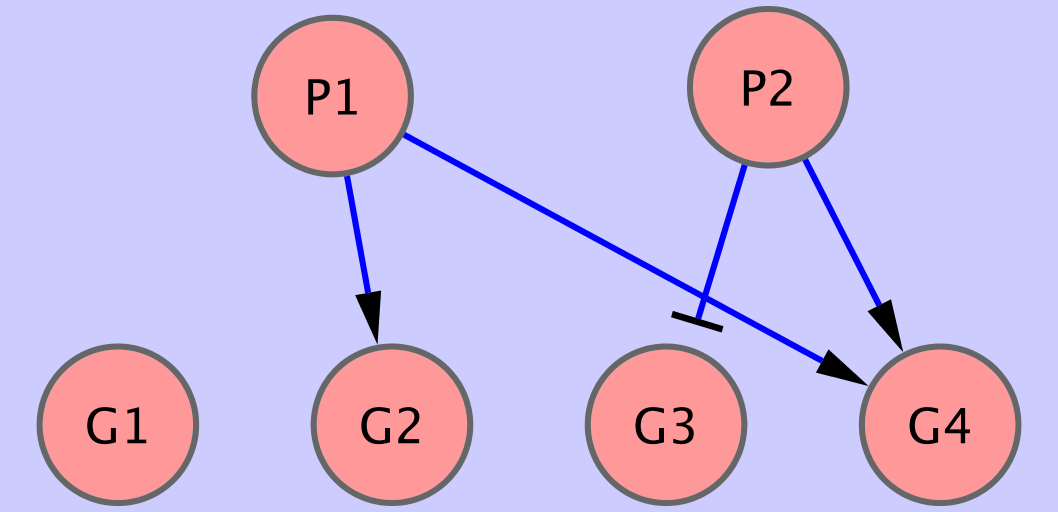
\includegraphics[width=8cm]{img/network1}  
  \caption{Very simple network consisting of 2 regulators and 4 observable regulatees.}
  \label{fig:net1}
\end{figure}

The first example shows how to use BNfinder to learn a simple static
Bayesian network. Let us imagine that we are analysisng cells under
two conditions $P1$ and $P2$ and that we are interested whether any of
the four genes: $G1,G2,G3,G4$ are responding to these conditions. We
assume that the true network is depicted in Fig \ref{fig:net1}, i.e. 
\begin{itemize}
\item $G1$ is not dependent on $P1$ or $P2$,
\item $G2$  is more likely to be expressed under condition $P1$,
\item $G3$ is less  likely to be expressed under condition $P2$,
\item $G4$ is more likely to  be expressed under any of the conditions $P1$ or $P2$.
\end{itemize}

We have collected 100 datapoints from this network, each consisting of
both the state of conditions and the discrete state of expression of
the genes. You can download the input file here \url{data/input1.txt}.

If you open the file in a text editor, please note that the first line
contains the information on the assumed structure:
\begin{verbatim}
#regulators P1 P2
\end{verbatim}
This represents the fact, that we assume that genes ($G1..G4$) can
depend on conditions ($P1,P2$) and not the other way around.

You can try to run BNfinder on this file:
\begin{verbatim}
bnf -e input1.txt -n output1.sif -v
\end{verbatim}
and you will see, that the network topology is reconstructed
properly. Also the orientation of the regulatory interactions is
inferred properly as you can see in the output file
\url{data/output1.sif}.

You can also try to see whether the optimal network is representative
for a larger set of possible suboptimal networks:
\begin{verbatim}
bnf -e input1.txt -n output1w.sif -v -i 4 -t output1.txt
\end{verbatim}
This time, in the output file (\url{data/output1w.sif}), the edge
labels represent the relative weights of different edges. In the file
\url{data/output1.txt}, we can find the originally computed weights
(i.e. relative probabilities -- see manual for details)
for all considered suboptimal sets of parents for all genes.

Instead of fixing the number of returned parents sets 
(option \texttt{-i 4}) you can specify thresholds for their weights
and/or weight ratios to optimal weights.
For example, if you wish to get for each vertex $v$
all parents sets with weights $>\max(0.1,0.01\cdot w_{opt}(v))$, 
where $w_{opt}(v)$ denotes the weight of the optimal parents set of $v$, 
you can type:
\begin{verbatim}
bnf -e input1.txt -n output1a.sif -v -i -1 -m 0.1 -o 0.01 -t output1a.txt
\end{verbatim}

We can also try to analyze the data for this network without
discretization: \url{data/input2.txt}. In this case we need another
directive to indicate that some of the dataseries are continuous:
\begin{verbatim}
#continuous G1 G2 G3 G4
\end{verbatim}

Again if we run BNfinder on this data, 
\begin{verbatim}
bnf -e input2.txt -n output2.sif -v
\end{verbatim}
we can verify, that the output file contains correct information \url{data/output2.sif}.

\subsubsection{Simple dynamic network}
\label{sec:simdyn}

BNfinder can be used also to infer dynamic Bayesian networks from time
series data. In this case it is not necessary to specify the
regulators sets, because DBNs, unlike static networks do not need to
be acyclic.

In the first dataset: \url{data/input3.txt}, we have 1 serie of 20
consecutive measurements of gene expression from gene network depicted
in Fig. \ref{fig:net2}.

\begin{figure}[h]
  \centering
  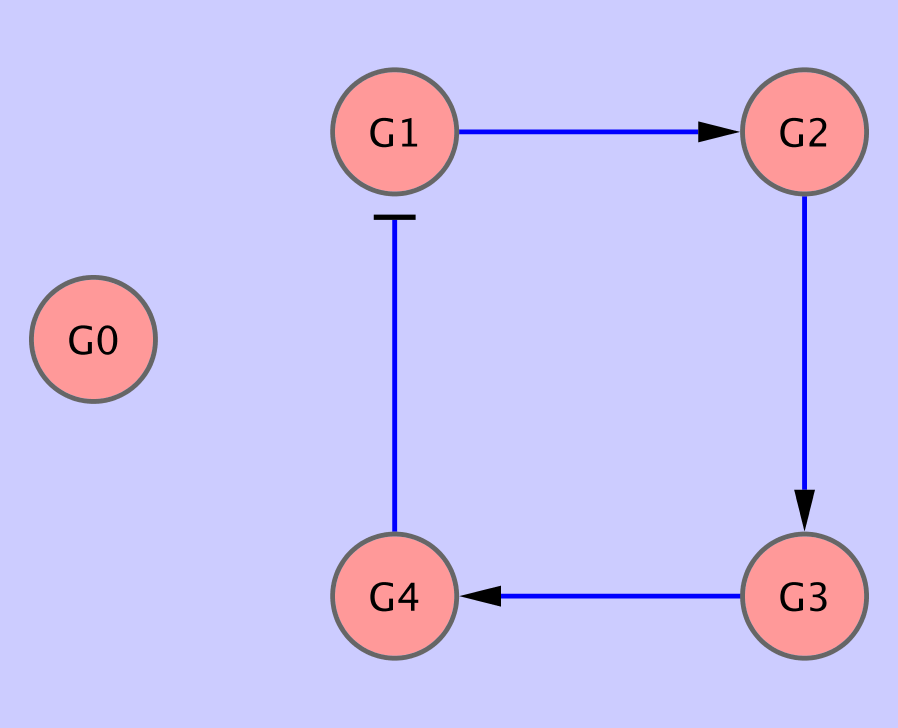
\includegraphics[width=8cm]{img/network2}  
  \caption{Very simple dynamic network consisting of 5 observables}
  \label{fig:net2}
\end{figure}

If we run BNfinder on this data:
\begin{verbatim}
bnf -e input3.txt -n output3.sif -v 
\end{verbatim}
We can see that the program was unable to correctly reconstruct all
the edges. Again, if we look at the statistics of edge occurences in
suboptimal networks,
\begin{verbatim}
bnf -e input3.txt -n output3.sif -v -i 10 -t output3.txt
\end{verbatim}
we can see that the correct edges are the most commonly occuring ones,
but they score lower than empty parent sets.

In this case we can show how perturbational data can be integrated
into this framework. We have collected gene expression from 5
time-series containing one single gene knockout for each of the genes:
\url{data/input4.txt}. The perturbations are noted by including the
following lines in the preamble of the data file:
\begin{verbatim}
#perturbed EXP1 G1
#perturbed EXP2 G2
#perturbed EXP3 G3
#perturbed EXP4 G4
#perturbed EXP5 G0
\end{verbatim}

If we run BNfinder on the perturbed data, we can see that all the edges
are reconstructed with high confidence.
\begin{verbatim}
bnf -e input4.txt -n output4.sif -v -i 10 -t output4.txt
\end{verbatim}

\subsubsection{Setting priors}
\label{sec:simprio}
\begin{figure}[h]
  \centering
  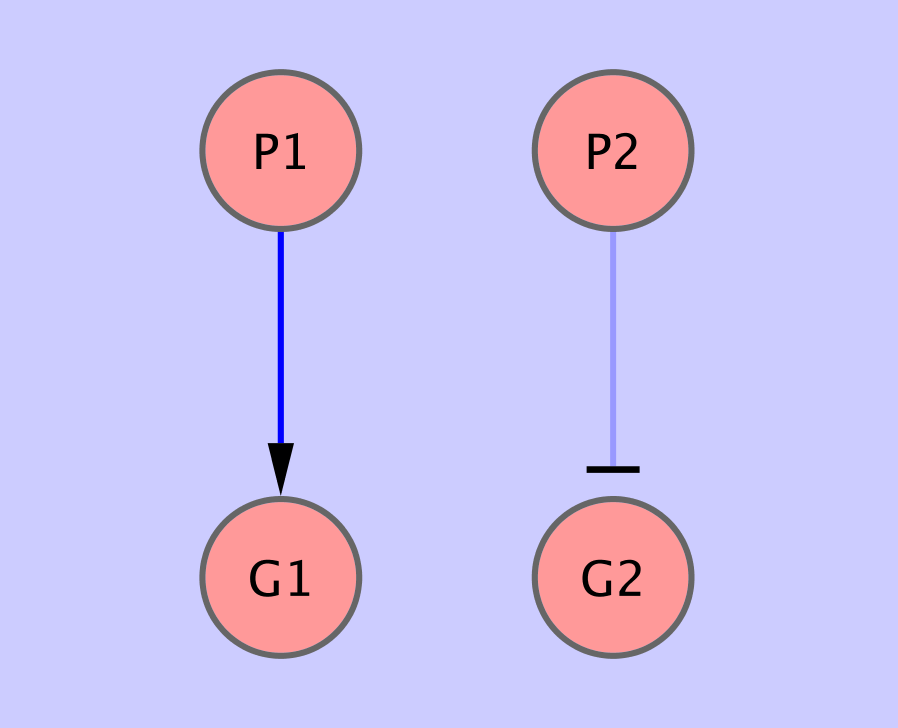
\includegraphics[width=6cm]{img/network3}  
  \caption{Exemplary network containing dependencies of different strength}
  \label{fig:net3}
\end{figure}
In some cases it might be useful to include some prior information on
the network structure into the process of inference. We will
illustrate this on an example of a simple network similar to the one
described in section \ref{sec:simstat}. This time it is an even
simpler network, with 2 conditions and 2 genes as depicted in
Fig. \ref{fig:net3}. Even though topology of the network is very
simple, the problem lies in the fact that the dependence of $G2$ on
$P2$ is weaker than the dependence of $G1$ on $P1$. This is why if we
run our software on the unmodified dataset \url{data/input5.txt}, 
\begin{verbatim}
bnf -e input5.txt -n output5.sif -v  -i 10 -t output5.txt
\end{verbatim}
we can see that the program is unable to recover the $P2\rightarrow G2$
edge. However, if we expect that $G2$ is  responding weakly to its regulators, 
we can increase the prior probability of $G2$ being regulated by any of 
the factors $P1,P2$ via decreasing its weight:
\begin{verbatim}
#prioredge G2 0.33 P2 P1
\end{verbatim}
We can see the edge appearing in the result as expected (see \url{data/input6a.txt}):
\begin{verbatim}
bnf -e input6a.txt -n output6a.sif -v  -i 10 -t output6a.txt
\end{verbatim}

Similarly, if we expect, that in general gene response to condition $P2$ is weaker, we may modify the prior probability of the condition $P2$ to be a regulator:
\begin{verbatim}
#priorvert 0.33 P2 
\end{verbatim}

The result of running BNFinder with this input (\url{data/input6b.txt}) is very similar to the previous one:
\begin{verbatim}
bnf -e input6b.txt -n output6b.sif -v  -i 10 -t output6b.txt
\end{verbatim}

\subsection{Examples of published  datasets}
\label{sec:real}

In this section, we present two more realistic examples of published
datasets used for inference of Bayesian networks. The first one
consists of measurements of states of protein signalling network under
different perturbations \cite{pmid15845847}. It's been used to infer
causal relationships in the form of static Bayesian network.

The second dataset comes from documentation of the Banjo package
\cite{Smith2006} which can be downloaded from
(\url{http://www.cs.duke.edu/$\sim$amink/software/banjo}). It consists
of 2000 observations describing a relatively large dynamic network
consisting of 20 nodes. It may be considered a benchmark of the
efficiency of our algorithm.

The third dataset is converted from an example attached to the
globalMIT software for Bayesian network reconstruction. It is similar
to the second example as it is also generated from a dynamic Bayesian
network and consists of 2000 observations of 20 variables. However, in
this case the variables are much less interconnected and there are
many self-regulatory loops.

\textbf{PLEASE NOTE that these datasets are too large to be run through BNFinder webserver. If you would like to run them, please download the software. }

\subsubsection{Static Protein signalling network}
\label{sec:realStat}

In this section we present how BNfinder can be applied to a protein
signalling network analyzed by Sachs et al \cite{pmid15845847}. We
took the data from the article, and transformed it into the format
suitable for BNfinder. We also needed to specify several properties of
the data in the preamble of the file \url{data/sachs.inp}

\begin{figure}[h]
  \centering
  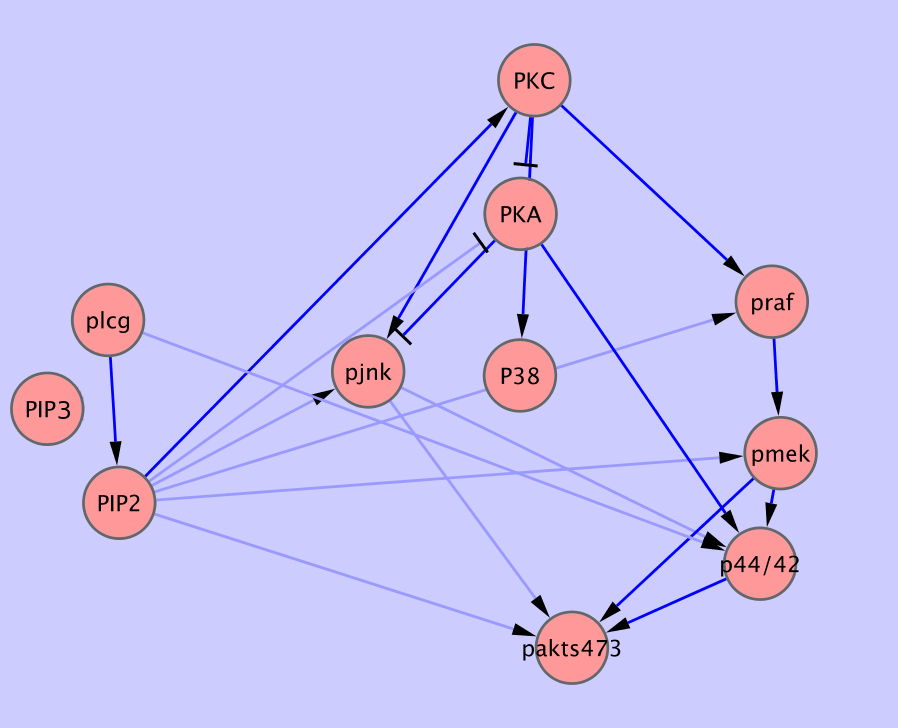
\includegraphics[width=8cm]{img/static}  
  \caption{Reconstruction of the protein signalling network. Dark blue
    arrows represent dependencies found in literature. Light blue
    arrows represent dependencies found by BNfinder but not expected
    by Sachs et al. \cite{pmid15845847}}
  \label{fig:stat}
\end{figure}

Firstly, we needed to specify that the data are continuous measurements:

\begin{verbatim}
#continuous praf pmek plcg PIP2 PIP3 p44/42 pakts473 PKA PKC P38 pjnk
\end{verbatim}

Then, we needed to specify the expected layer structure of the signalling pathway we are studying:
\begin{verbatim}
#regulators plcg
#regulators PIP3
#regulators PIP2
#regulators PKC
#regulators PKA
#regulators praf
#regulators pjnk pmek P38 
#regulators p44/42
#regulators pakts473
\end{verbatim}

Then we needed to specify which of the proteins are affected by different perturbations. 
\begin{verbatim}
#perturbed cd3cd28psitect_0 PIP2
#perturbed cd3cd28psitect_1 PIP2
#perturbed cd3cd28psitect_2 PIP2
...
#perturbed cd3cd28g0076_0 PKC
#perturbed cd3cd28g0076_1 PKC
#perturbed cd3cd28g0076_2 PKC
...
\end{verbatim}

When we finally run the BNfinder:
\begin{verbatim}
bnf -e sachs.inp -n sachs.sif -v 
\end{verbatim}
We obtain the network presented in Fig. \ref{fig:stat}. As we can see,
the topology is quite consistent with the literature data. Out of 17
expected edges, BNfinder recovers 11 correctly. 

\subsubsection{Dynamic Bayesian network}
\label{sec:realDyn}

This is a dataset of substantial size which is used  \cite{bnfinder} to
assess the performance of our inference algorithm. The input dataset
(\url{data/input7.txt}{}) consists of 2000 measurements of 20 variables
and it takes approximately 3 hours to compute it on a modern PC (2.4Ghz
Intel Core 2 duo). 

We can run BNfinder with the following command (note that we are
using the \texttt{-l} option to limit the number of parents to $5$):
\begin{verbatim}
bnf -e input7.txt -n output7.sif -v -l 5 -txt output7.txt
\end{verbatim}

In Fig. \ref{fig:dyn} we can see part of the network reconstructed by
BNfinder. All the edges reported by Banjo are also present in the
optimal network (dark blue). The optimal network contains a number of
additional edges, not reported by Banjo.

\begin{figure}[h]
  \centering
   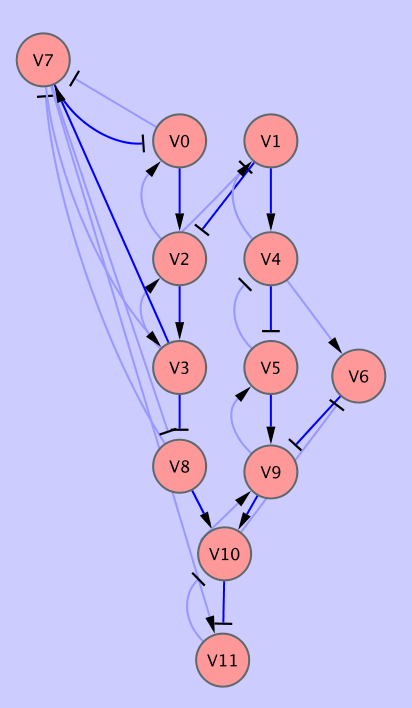
\includegraphics[width=5cm]{img/dynamic}  
  \caption{The optimal network reconstructed by BNfinder from the dynamic benchmark
    dataset. The edges reported also by Banjo are shown in dark blue. }
  \label{fig:dyn}
\end{figure}

If you want to see how much faster the MDL algorithm is, you can also run BNfinder 
with the following command:
\begin{verbatim}
bnf -s MDL -e input7.txt -n output7mdl.sif -v -l 5 -txt output7mdl.txt
\end{verbatim}

\subsubsection{Dynamic network containing self-regulatory loops}
\label{sec:self-loops}

In this example, we can utilize both the \texttt{-g 1} option for
allowing self-regulations as well as the \texttt{-s MIT} option for
using the MIT score.

\begin{verbatim}
bnf -s MIT -e input8.txt -n output8.sif -v -l 3 -txt output8.txt -c output8.cpd -g 1
\end{verbatim}

One additional parameter that is unique to the MIT score is the
significance level $\alpha$ of the $\chi^2$ distribution
(\texttt{-a}). The default level for $\alpha$ is $.9999$, but we can
increase/decrease it if we want to see fewer/more edges respectively.

For example, setting the level alpha to a higher value should give us more edges in the result:

\begin{verbatim}
bnf -s MIT -e input8.txt -n output8.sif -v -l 3 -a .9  -g 1
\end{verbatim}

\subsubsection{Using multiple processors for faster computations}
\label{sec:multicore}

Since most current computers are equipped with multiple processors, we
can take advantage of that fact to speed up BNFinder
computation. Especially for large datasets, such as the ones described
in previous sections, we can take full advantage of the parallell
computation. For example, if we want BNfinder to run on 4 CPUs in
parallell, we can use the \texttt{-k 4} option as in the following example:

\begin{verbatim}
bnf -s MIT -e input8.txt -n output8.sif -v -l 3 -a .9  -g 1 -k 4
\end{verbatim}


\subsection{Example of classification with BNfinder}

\texttt{bnf-cv} and \texttt{bnc} tools can be used to solve classification tasks with classifier based on Bayesian networks. The former is used to perform a cross-validation test and the later to classify a dataset when you already have a classifier. In our example we will try to solve the following problem: we have points within the unit square; our positive set consists of those that are located in top-right and bottom-left corners, i.e. x + y > 1.8 or x + y < 0.2. The training set consists of 100 positive and 100 negative examples. They are visualised in the following Fig. \ref{fig:training}. The data can be downloaded from here (\url{data/training\_set.txt}). We marked x and y as continuous regulators. We will classify only one feature, but it is possible to perform cross-validation and classification procedure for more variables. All variables not marked as regulators are treated as variables to be explained by classifier.

\begin{figure}[h]
  \centering
   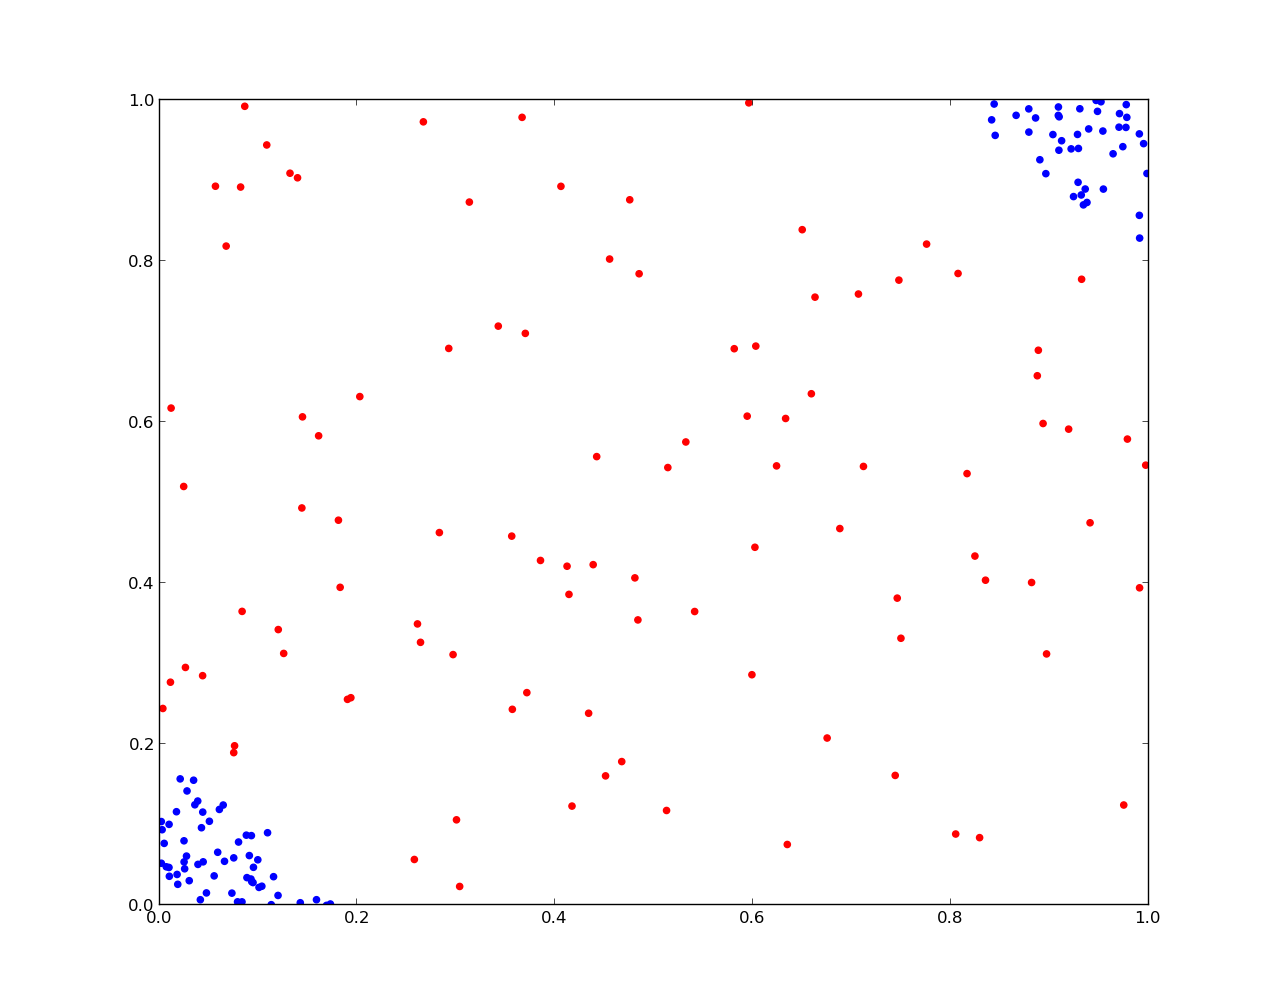
\includegraphics[width=10cm]{img/training}
  \caption{The training set used in the classification example. Positive examples are colored blue. }
  \label{fig:training}
\end{figure}

To perform a 10-fold cross-validation we can use the following command:
\begin{verbatim}
bnf-cv -e training_set.txt -c net.cpd -k 10 -r ROC.pdf
\end{verbatim}

As a result we obtain 10 files (net.cpd0, net.cpd1, ..., net.cpd9) containing networks in cpd format corresponding to respective folds of the cross-validation. Every execution of foregoing command will bring different results, because a split into 10 sets is done randomly. In the result file ROC.pdf there is a ROC plot showing the results of cross-validation (see \ref{fig:ROC}). Further results are printed to the standard output and contains (among others) information about regulators taken to each of 10 classifiers and AUC measure of each classifier's performance. 

\begin{figure}[h!]
  \centering
   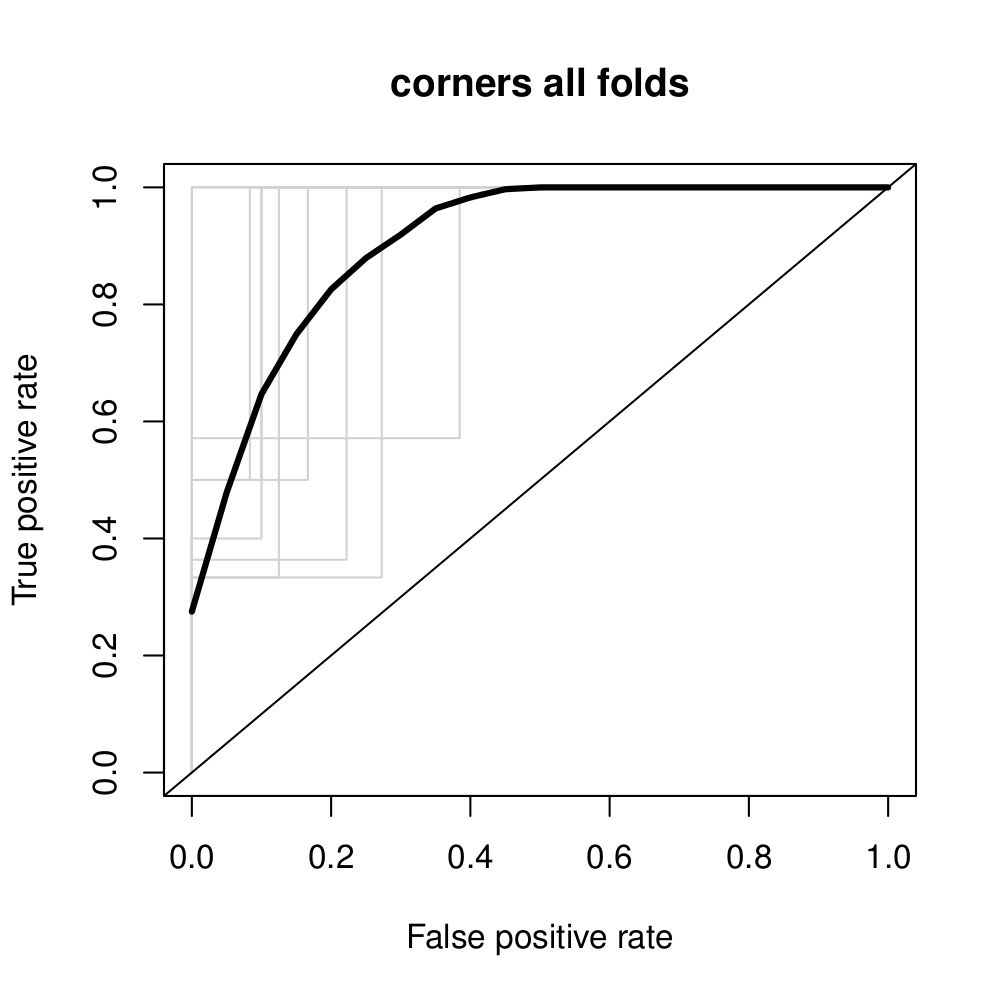
\includegraphics[width=10cm]{img/ROC}
  \caption{The Receiver operating characteristics curve for 10-fold cross-validation. The thick curve shows the average performance of classifiers. }
  \label{fig:ROC}
\end{figure}

To perform classification task on a test dataset we can use any of the nets obtained from cross-validation task but usually it is better to train a classifier on the whole training dataset. It can be done by the following command:
\begin{verbatim}
bnf -e training_set.txt -c net.cpd
\end{verbatim}

We will test out classifier on this (\url{data/test\_set.txt}) dataset which consists of 1000 points from the unit square. Now, by using the \texttt{bnc} tool we can obtain the classification. In the Fig. \ref{fig:classificationresult} we can see the result of classifying our test dataset by classifier in the file net.cpd (we used 0.63 probability threshold to generate the plot):
\begin{verbatim}
bnc -o result.cls -p 1 -c net.cpd -d test_set.txt
\end{verbatim}

\begin{figure}[h!]
  \centering
   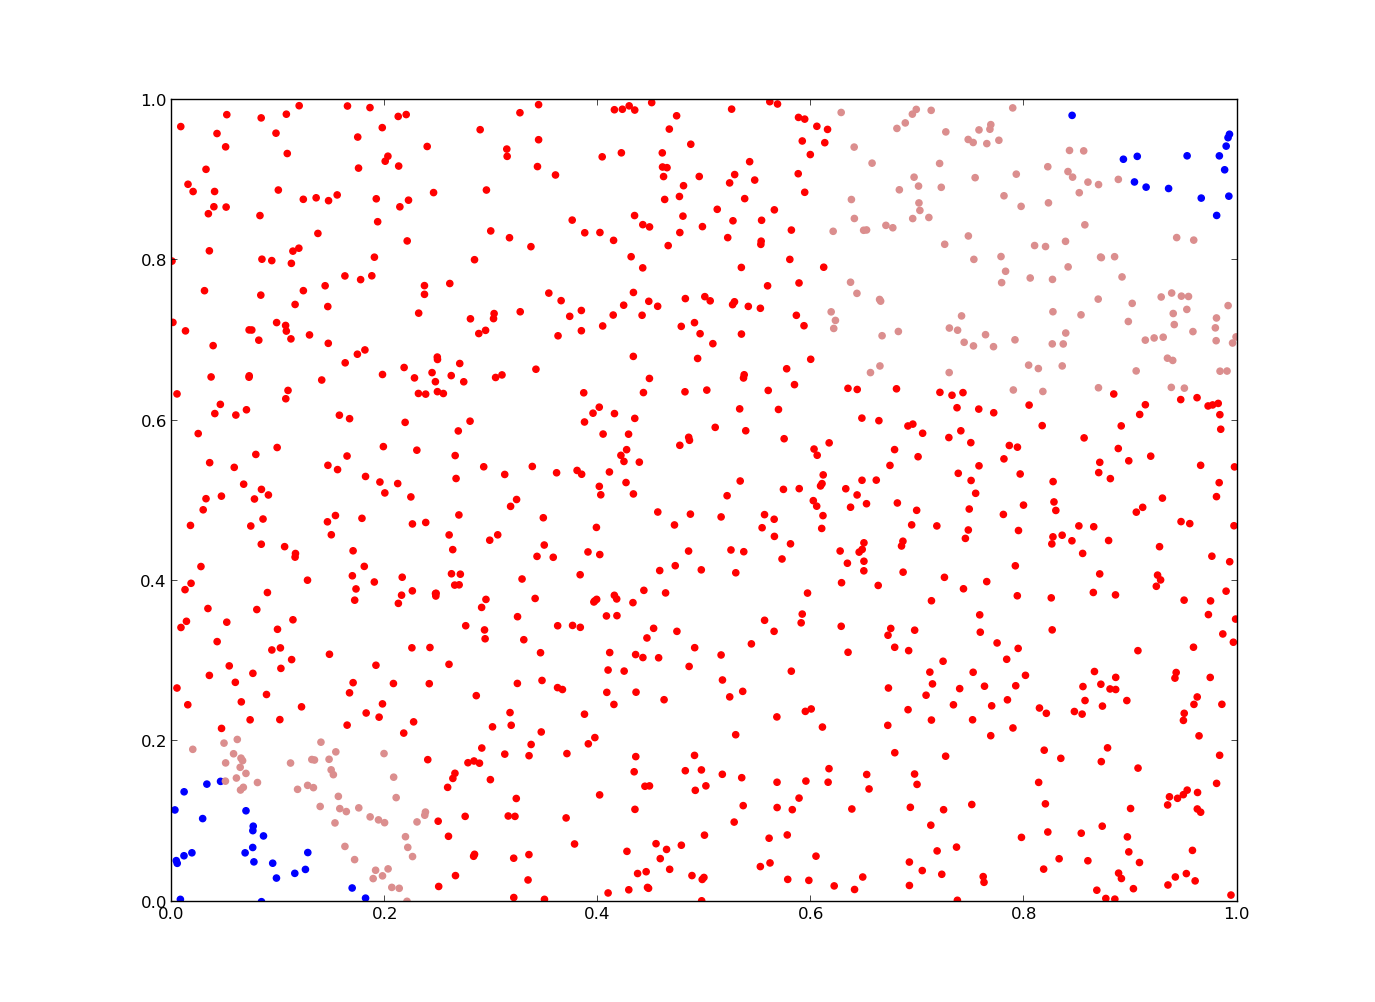
\includegraphics[width=10cm]{img/classificationresult}
  \caption{The result of classification. Blue and red points represent true positives and negatives. There was no false negatives. False positives are colored light red.}
  \label{fig:classificationresult}
\end{figure}

We can also find the most probable class for \texttt{corners} for every experiment by executing:
\begin{verbatim}
bnc -o result.cls -m 1 -c net.cpd -d test_set.txt
\end{verbatim}

Finally, by executing
\begin{verbatim}
bnf-cv -e training_set.txt -k 1 -r ROC.pdf
\end{verbatim}
command one can generate a colored plot of classifier trained on the whole training set. Different colors (explained on the right side of the picture) indicate probability thresholds above which we classify example as a positive one. An example of such a plot can be seen on the Fig. \ref{fig:rock1}.

\begin{figure}[h!]
  \centering
   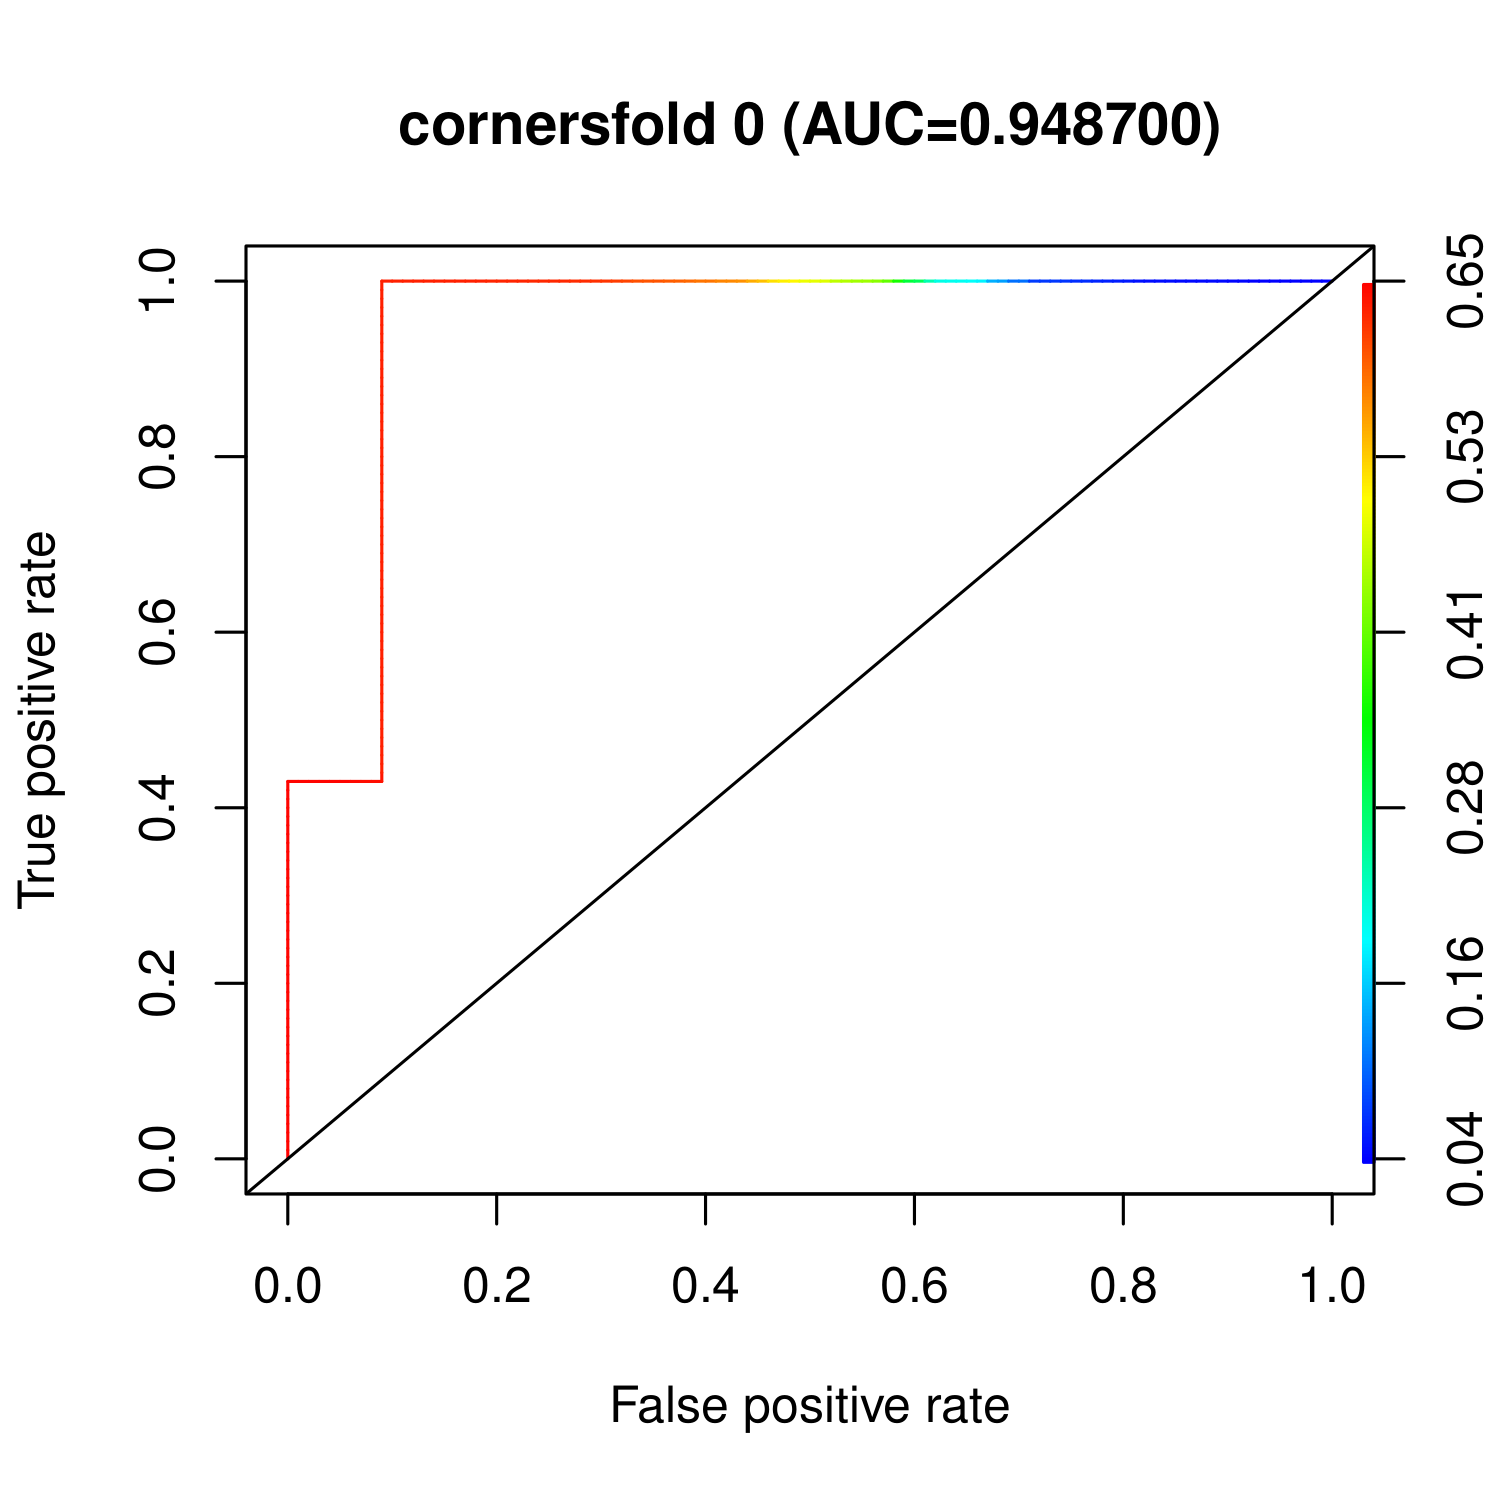
\includegraphics[width=10cm]{img/rock1}
  \caption{The effect of ploting ROC curve from 1-fold cross-validation.}
  \label{fig:rock1}
\end{figure}

%%% Local Variables: 
%%% mode: latex
%%% TeX-master: "tut"
%%% End: 


\section{Supplementary methods}
 In the present section we give a brief exposition of the algorithm implemented in BNFinder and its computational cost for two generally used scoring criteria: Minimal Description Length and Bayesian-Dirichlet equivalence.
 For a fuller treatment, including detailed proofs, we refer the reader to
%   \cite{dojer06}.
     \cite{dojer06,dojer10}.

\subsection{Polynomial-time exact algorithm}

 A \emph{Bayesian network} (BN) $\N$ is a representation of a joint distribution of a set of discrete random variables $\X=\{X_1,\ldots,X_n\}$.
 The representation consists of two components:
 \begin{itemize}
  \item a directed acyclic graph $\G=(\X,\E)$ encoding conditional (in-)dependencies
  \item a family $\theta$ of conditional distributions $P(X_i|\Pa_i)$, where
   $$\Pa_i=\{Y\in\X|(Y,X_i)\in\E\}$$
 \end{itemize}
 The joint distribution of $\X$ is given by
 \begin{equation}\label{joinprob}
 P(\X)=\prod_{i=1}^n P(X_i|\Pa_i)
 \end{equation}

 The problem of learning a BN is understood as follows: 
 given a multiset of $\X$-instances $\D=\{\x_1,\ldots,\x_N\}$ find a network graph $\G$ that best matches $\D$.
 The notion of a good match is formalized by means of a \emph{scoring function} $S(\G:\D)$ having positive values and minimized for the best matching network. 
 Thus the point is to find a directed acyclic graph $\G$ with the set of vertices $\X$ minimizing $S(\G:\D)$.
 
 The BNFinder program is devoted to the case when there is no need to examine the acyclicity of the graph, for example:
 \begin{itemize}
  \item When dealing with \emph{dynamic} Bayesian networks. A dynamic BN  describes stochastic evolution of a set of random variables over discretized time. Therefore conditional distributions refer to random variables in neighboring time points. The acyclicity constraint is relaxed, because the ''unrolled'' graph (with a copy of each variable in each time point) is always acyclic (see \cite{friedman98} for more details). The following considerations apply to dynamic BNs as well. 
  \item In case of static Bayesian Networks, the user has to supply the
   algorithm with a partial ordering of the vertices, restricting the
   set of possible edges only to the ones consistent with the
   ordering. BNFinder lets the user to divide the set of variables into an
   ordered set of disjoint subsets of variables, where edges can only
   exist between variables from different subsets and they have to be
   consistent with the ordering. If such ordering is not known
   beforehand, one can try to run BNFinder with different orderings and
   choose a network with the best overall score.
 \end{itemize}
 
 %The detailed description of the most generally used MDL and BDe scores will be provided in further sections.
 In the sequel we consider some assumptions on the form of a scoring function.
 The first one states that $S(\G:\D)$ decomposes into a sum over the set of random variables of \emph{local scores}, depending on the values of a variable and its parents in the graph only.
 
\begin{ass}[additivity]\label{as1}
 $S(\G:\D) = \sum_{i=1}^n s(X_i,\Pa_i:\D|_{\{X_i\}\cup\Pa_i})$, where $\D|_{\Y}$ denotes the restriction of $\D$ to the values of the members of $\Y\subseteq\X$.
\end{ass}

 When there is no need to examine the acyclicity of the graph, this assumption allows to compute the parents set of each variable independently.
 Thus the point is to find $\Pa_i$ minimizing $s(X_i,\Pa_i:\D|_{\{X_i\}\cup\Pa_i})$ for each $i$.

 Let us fix a dataset $\D$ and a random variable $X$. 
 We denote by $\X'$ the set of potential parents of $X$ (possibly smaller than $\X$ due to given constraints on the structure of the network).
 To simplify the notation we continue to write $s(\Pa)$ for $s(X,\Pa:\D|_{\{X\}\cup\Pa})$.
 
 The following assumption expresses the fact that scoring functions decompose into 2 components: $g$ penalizing the complexity of a network and $d$ evaluating the possibility of explaining data by a network.

\begin{ass}[splitting]\label{as2}
 $s(\Pa)=g(\Pa)+d(\Pa)$ for some functions $g,d:\mathcal{P}(\X)\to\mathbb{R}^+$ satisfying $\Pa\subseteq\Pa'\Longrightarrow g(\Pa)\le g(\Pa')$.
\end{ass}

 This assumption is used in the following algorithm to avoid considering networks with inadequately large component $g$.

\begin{alg}\label{a1}~
\begin{center}
\begin{tabular}{|p{0.9\textwidth}|}\hline
\begin{enumerate}
\item $\Pa:=\emptyset$
\item for each $\PP\subseteq\X'$ chosen according to $g(\PP)$
\begin{enumerate}
\item if $s(\PP)<s(\Pa)$ then $\Pa:=\PP$
\item if $g(\PP)\ge s(\Pa)$ then return $\Pa$; stop
\end{enumerate}
\end{enumerate}\\
\hline
\end{tabular}
\end{center}
\end{alg}

 In the above algorithm \emph{choosing according to $g(\PP)$} means choosing increasingly with respect to the value of the component $g$ of the local score.
 
 \begin{theorem}
 Suppose that the scoring function satisfies Assumptions \ref{as1}-\ref{as2}. Then Algorithm \ref{a1} applied to each random variable finds an optimal network.
 \end{theorem}
 
 A disadvantage of the above algorithm is that finding a proper subset $\PP\subseteq\X'$ involves computing $g(\PP')$ for all $\subseteq$-successors $\PP'$ of previously chosen subsets. 
 It may be avoided when a further assumption is imposed.

\begin{ass}[uniformity]\label{as3}
 $|\Pa|=|\Pa'|\Longrightarrow g(\Pa)=g(\Pa')$.
\end{ass}

 The above assumption suggests the notation $\g(|\Pa|)=g(\Pa)$. 
 The following algorithm uses the uniformity of $g$ to reduce the number of computations of the component $g$.

\begin{alg}\label{a2}~
\begin{center}
\begin{tabular}{|p{0.9\textwidth}|}\hline
\begin{enumerate}
\item $\Pa:=\emptyset$
\item for $p=1$ to $n$%$|\X|$
\begin{enumerate}
\item if $\g(p)\ge s(\Pa)$ then return $\Pa$; stop
\item $\PP=arg min_{\{\Y\subseteq\X' : |\Y|=p\}}s(\Y)$
\item if $s(\PP)<s(\Pa)$ then $\Pa:=\PP$
\end{enumerate}
\end{enumerate}\\
\hline
\end{tabular}
\end{center}
\end{alg}

 \begin{theorem}
 Suppose that the scoring function satisfies Assumptions \ref{as1}-\ref{as3}. Then Algorithm \ref{a2} applied to each random variable finds an optimal network.
 \end{theorem}
 
\subsection{Minimal Description Length}

 The Minimal Description Length (MDL) scoring criterion originates from information theory \cite{lam94}. 
 A network $\N$ is viewed here as a model of compression of a dataset $\D$. 
 The optimal model minimizes the total length of the description, i.e. the sum of the description length of the model and of the compressed data.
 MDL is effectively equivalent to Bayesian Information Criterion (BIC) 
 (see \cite{neapolitan03}), 
 which approximates Bayesian scores (see next section) 
 and is also applicable to continuous data.

 Let us fix a dataset $\D=\{\x_1,\ldots,\x_N\}$ and a random variable $X$. 
 Recall the decomposition $s(\Pa)=g(\Pa)+d(\Pa)$ of the local score for $X$. 
 In the MDL score $g(\Pa)$ stands for the length of the description of the local part of the network (i.e. the edges ingoing to $X$ and the conditional distribution $P(X|\Pa)$) and $d(\Pa)$ is the length of the compressed version of $X$-values in $\D$.
 
 Let $k_Y$ denote the cardinality of the set $\V_Y$ of possible values of the random variable $Y\in\X$.
 Thus we have 
 $$g(\Pa)=|\Pa|\log n+\frac{\log N}{2}(k_X-1)\prod_{Y\in\Pa}k_Y$$
 where $\frac{\log N}{2}$ is the number of bits we use for each numeric parameter of the conditional distribution. 
 This formula satisfies Assumption \ref{as2} but fails to satisfy Assumption \ref{as3}.
 Therefore Algorithm \ref{a1} can be used to learn an optimal network, but Algorithm \ref{a2} cannot. 
 
 However, for many applications we may assume that 
 all random variables have the same value set $\V$ of cardinality $k$.
 In this case we obtain the formula
 $$g(\Pa)=|\Pa|\log n+\frac{\log N}{2}(k-1)k^{|\Pa|}$$
 which satisfies Assumption \ref{as3}.
 For simplicity, we continue to work under this assumption.
 
 Compression with respect to the network model is understood as follows: when encoding the $X$-values, the values of $\Pa$-instances are assumed to be known. 
 Thus the optimal encoding length is given by 
 $$d(\Pa)=N\cdot H(X|\Pa)$$
 where $H(X|\Pa)=-\sum_{v\in\V}\sum_{\vp\in\V^{\Pa}}P(v,\vp)\log P(v|\vp)$ is the conditional entropy of $X$ given $\Pa$ (the distributions are estimated from $\D$).
 
 Since all the assumptions from the previous section are satisfied, Algorithm \ref{a2} may be applied to learn the optimal network. 
 Let us turn to the analysis of its complexity.
 
 \begin{theorem}
 The worst-case time complexity of Algorithm \ref{a2} for the MDL score is $\OO(n^{\log_k N}N\log_k N)$.
 \end{theorem}
 
\subsection{Bayesian-Dirichlet equivalence}

 The Bayesian-Dirichlet equivalence (BDe) scoring criterion originates from Bayesian statistics \cite{cooper92}. 
 Given a dataset $\D$ the optimal network structure $\G$ maximizes the \emph{posterior} conditional probability $P(\G|\D)$. 
 We have 
 $$P(\G|\D)\propto P(\G)P(\D|\G)=P(\G)\int P(\D|\G,\theta)P(\theta|\G)d\theta$$
 where $P(\G)$ and $P(\theta|\G)$ are \emph{prior} probability distributions on graph structures and conditional distributions' parameters, respectively, and $P(\D|\G,\theta)$ is evaluated due to \eqref{joinprob}.
 
 Heckerman et al. \cite{heckerman95}, following Cooper and Herskovits \cite{cooper92}, identified a set of independence assumptions making possible decomposition of the integral in the above formula into a product over $\X$.
 Under this condition, together with a similar one regarding decomposition of $P(\G)$, the scoring criterion
 $$S(\G:\D)=-\log P(\G)-\log P(\D|\G)$$
 obtained by taking $-\log$ of the above term satisfies Assumption \ref{as1}. 
 Moreover, the decomposition $s(\Pa)=g(\Pa)+d(\Pa)$ of the local scores appears as well, with the components $g$ and $d$ derived from $-\log P(\G)$ and $-\log P(\D|\G)$, respectively.

% The distribution $P((\X,\E))\propto\alpha^{|\E|}$ with a penalty parameter $0<\alpha<1$ in general is used as a prior over the network structures. 
% This choice results in the function 
% $$g(|\Pa|)=|\Pa|\log\alpha^{-1}$$ 
% satisfying Assumptions \ref{as2} and \ref{as3}.

 The distribution $P((\X,\E))\propto\prod_{e\in\E}\alpha_{e}$ 
 with penalty parameters $0<\alpha_e<1$ 
 is commonly used as a prior over the network structures. 
 BNFinder sets $\alpha_{(Y,X)}=1/k_Y$ by default.
 This choice results in the function 
 $$g(\Pa)=\sum_{Y\in\Pa}\log k_Y$$ 
 satisfying Assumptions \ref{as2}.
 If we moreover assume that all random variables 
 have the same value set $\V$ of cardinality $k$,
 we obtain the function
 $$g(\Pa)=|\Pa|\log k$$ 
 satisfying also Assumption \ref{as3}.
 For simplicity, we continue to work under this assumption.

 However, it should be noticed that there are also used priors 
 which satisfy neither Assumption \ref{as2} nor \ref{as3}, 
 e.g.  $P(\G)\propto\alpha^{\Delta(\G,\G_0)}$, 
 where $\Delta(\G,\G_0)$ is the cardinality of the symmetric difference 
 between the sets of edges in $\G$ and in the prior network $\G_0$.
 
 The \emph{Dirichlet distribution} is generally used as a prior over the conditional distributions' parameters.
 It yields
 $$d(\Pa)=\log\left(\prod_{\vp\in\V^{|\Pa|}}
  \frac{\Gamma(\sum_{v\in\V}(H_{v,\vp}+N_{v,\vp}))}{\Gamma(\sum_{v\in\V}H_{v,\vp})}
  \prod_{v\in\V}\frac{\Gamma(H_{v,\vp})}{\Gamma(H_{v,\vp}+N_{v,\vp})}\right)$$
 where $\Gamma$ is the \emph{Gamma} function, $N_{v,\vp}$ denotes the number of samples in $\D$ with $X=v$ and $\Pa=\vp$, and $H_{v,\vp}$ is the corresponding \emph{hyperparameter} of the Dirichlet distribution.
 
 Setting all the hyperparameters to $1$ yields
 \begin{multline*}d(\Pa)=\log\left(\prod_{\vp\in\V^{|\Pa|}}
  \frac{(k-1+\sum_{v\in\V}N_{v,\vp})!}{(k-1)!}
  \prod_{v\in\V}\frac{1}{N_{v,\vp}!}\right)=\\
  =\sum_{\vp\in\V^{|\Pa|}}\left(
 \log({\textstyle k-1+\underset{v\in\V}{\sum}N_{v,\vp}})!-\log(k-1)!
  -\sum_{v\in\V}\log{N_{v,\vp}!}\right)
 \end{multline*}
 where $k=|\V|$.
 For simplicity, we continue to work under this assumption (following Cooper and Herskovits \cite{cooper92}).
 The general case may be handled in a similar way.
 
 The following result allows to refine the decomposition of the local score into the sum of the components $g$ and $d$.
 
 \begin{proposition}
 Define $d_{min}=\sum_{v\in\V}\left(\log(k-1+N_v)!-\log(k-1)!-\log N_v!\right)$, where $N_v$ denotes the number of samples in $\D$ with $X=v$. 
 Then $d(\Pa)\ge d_{min}$ for each $\Pa\in\X$.
 \end{proposition}
 
 By the above proposition, the decomposition of the local score given by $s(\Pa)=g'(\Pa)+d'(\Pa)$ with the components $g'(\Pa)=g(\Pa)+d_{min}$ and $d'(\Pa)=d(\Pa)-d_{min}$ satisfies all the assumptions required by Algorithm \ref{a2}. 
 Let us turn to the analysis of its complexity.
  
 \begin{theorem}
 The worst-case time complexity of Algorithm \ref{a2} for the BDe score with the decomposition of the local score given by $s(\Pa)=g'(\Pa)+d'(\Pa)$ is $\OO(n^{N\log_{\alpha^{-1}}k}N^2\log_{\alpha^{-1}}k)$.
 \end{theorem}


\subsection{Mutual information test}

The Mutual Information Test (MIT) scoring criterion originates from the concept of mutual information, belonging to the family of measures based on information theory \cite{deCampos}. Briefly speaking, this method combines mutual information measure and a statistical independence test based on the chi-square dustribution assosiated with it. The goodness of a fit of the particular network is computed as the total mutual information between each node and its parents. This score is then penalized by a term corresponding to the degree of statistical significance of the shared information. 

Let $\mathcal{D}$ be a dataset with $N$ observations, $\mathcal{G}$ be the dynamic bayesian network. 
Let $X = \{X_1,...,X_n\}$ be the set of $n$ variables, with each of it corresponding to $ \{r_1,...,r_n$\} discrete states.
Let's denote the set of parents of $X_i$ in $\mathcal{G}$ with corresponding $\{r_{i1},...,r_{is_i}\}$ discrete states
as $\Pa_i = \{X_{i1},...,X_{is_i}\}$. 
Then the MIT score is defined as follows \cite{globMIT}: 
$$\mathcal{S(G:D)} = \sum_{i=0; \Pa_i \neq \emptyset}^n \{ 2N \cdot I(X_i, \Pa_i) - \sum_{j=1}^{s_i} \chi_{\alpha l_i \sigma_i(j)} \}$$

In this formula $I(X_i, \Pa_i)$ denotes the mutual information between $X_i$ and its parents
as estimated from $\mathcal{D}$ and defined as $$ I(X;Y) = \sum_{y \in Y} \sum_{x \in X} p(x,y) \log \left(\frac{p(x,y)}{p(x)p(y)}\right)  $$
$\chi_{\alpha l_i \sigma_i(j)} $ is the chi-square distribution at significance level $1-\alpha$.
It is defined as the value such that $$p(\chi^{2}(l_{ij}) \le \chi_{\alpha l_ij})=\alpha $$
\\The term $ l_{i \sigma_i (j)}$ denotes the degrees of freedom and is defined as 
$$ l_{i \sigma_i (j)} = \begin{cases}
   (r_i-1)(r_{i \sigma_i (j)} -1) \prod_{k=1}^{j-1} r_{i \sigma_i (k)}, & \text{$j=2..,s_i$}.\\
   (r_i-1)(r_{i \sigma_i (j)} -1), & \text{$j=1$}.
 \end{cases}
$$
where $\sigma_i = \{\sigma_i (1),...,\sigma_i(s_i)\}$ is any permutation of the index set
$\{1...s_i\}$ of $\Pa_i$ such that, the number of states of the variables
decreases with the increasing position in the permutation. 

Recall the decomposition $ S_{MIT}(\Pa_i) = d_{MIT}(\Pa_i) + g_{MIT}(\Pa_i) $. 
In this case:  
$$ d_{MIT}(\Pa_i) = 2N\cdot I(X_i, \mathbf{X}) - 2N \cdot I(X_i, \Pa_i) $$
$$ g_{MIT}(\Pa_i) = \sum_{j=1}^{s_i} \chi_{\alpha l_i \sigma_i(j)} $$ 
Roughly, $d_{MIT}$ measures the accuracy of representing the joint distribution of 
$\mathcal{D}$ by $\mathcal{G}$ while $g_{MIT}$ measures the complexity of this representation. This decomposition
satisfies Assumption 2.
However, MIT score defined in this way does not satisfy Assumption 3.
Therefore, we introduce an assumption that all the variables have the same number of discrete states.

\begin{ass}[uniformity]\label{as4}
 All variables in $X$ have the same number of discrete states k.
\end{ass}

Under this assumption it can be easily shown that $g_{MIT}$ satisfies Assumption 3.
 \begin{theorem} \cite{globMITManual}
 The worst-case time complexity of Algorithm \ref{a2} for the MIT score under the assumption of the variables uniformity is polynomial in the number of variables. 
 \end{theorem}


\subsection{Continuous variables}

All the scoring functions implemented in BNFinder (MDL, BDe and MIT) 
were originally designed for discrete variables.
In order to avoid arbitrary discretization of continuous data 
we adapted them to deal with continuous variables directly. 
Moreover, our method works also with heterogenous data sets 
joining together discrete and continuous variables.

%% The distribution of each continuous variable is assumed to be 
%% a mixture of two normal distributions.
%% Mixture parameters are estimated from data clustered with the \emph{k-means} algorithm 
%% ($k=2$, cutting the set of variable values in the median yields the initial clusters).
%% Then the parameters are used in transforming continuous values into 
%% probability distributions on the mixture components.
%% These components are considered to be the two possible values 
%% (\emph{low} and \emph{high}) 
%% of a related hidden discrete variable.

The distribution of each continuous variable $X$ is assumed to be 
a mixture of two normal distributions.
Mixture components correspond to the two possible values 
(\emph{low} and \emph{high}) of a related hidden discrete variable $X'$
and $X$ is viewed as its observable reflection.
%Therefore regulatory relationships are learned 
%for discrete variables rather than continuous ones.
Consequently, the conditional distributions of $X$ is given by:
%\begin{multline*}
$$
P(X|\Pa)=
\sum_{v\in\Vc}\sum_{\vp\in\Vc^{|\Pa|}}P(X|X'=v)P(X'=v|\Pa'=\vp)P(\Pa'=\vp|\Pa)
$$
%=\\
%=\sum_{v\in\Vc}
%\left(\sum_{\vp\in\Vc^{|\Pa|}}P(X'=v|\Pa'=\vp)P(\Pa'=\vp|\Pa)\right)
%P(X|X'=v)
%\end{multline*}
%Since distributions $P(X|X'=v)$ are Gaussian, 
%$P(X|\Pa)$ is a Gaussian mixture with parameters dependent on values of $\Pa$.

%In a preprocessing step parameters of $P(X|X')$ are estimated separately 
%for each variable $X$.
Conditional distributions $P(X|X')$ are assumed to be independent 
for all variables $X$.
Thus we estimate their parameters separately for each $X$ in a preprocessing step.
Estimation is based on data clustering with the \emph{k-means} algorithm 
($k=2$, cutting the set of variable values in the median yields initial clusters).
Due to the independence assumption, these parameters enable us to calculate also
$P(\Pa'|\Pa)=\prod_{Y\in\Pa}P(Y'|Y)$.
Thus the space of possible conditional distributions on continuous variables
forms a family of Gaussian mixtures, parameterized by $P(X'|\Pa')$, 
%They are the only free parameters in $P(X|\Pa)$ and at the same time the parameters of
conditional distributions on corresponding discrete variables.

From a technical point of view,
BNFinder learns optimal network structures for these discrete variables, 
using scoring functions adapted to handle 
distributions on variable values instead of their determined values
(expected values of original scores are computed).
For continuous variables it gives optimal Bayesian networks from among 
all networks with conditional probability distributions
belonging to the above defined family of Gaussian mixtures.


The following results present the complexity of our algorithm 
with continuous MDL and BDe scoring functions.

 \begin{theorem}
 The worst-case time complexity of Algorithm \ref{a2} for the continuous MDL score is $\OO(n^{\log N}N^2)$.
 \end{theorem}
 
 \begin{theorem}
 The worst-case time complexity of Algorithm \ref{a2} for the continuous BDe score with the decomposition of the local score given by $s(\Pa)=g'(\Pa)+d'(\Pa)$ is $\OO((2n)^\frac{N}{\log\alpha^{-1}}N)$.
 \end{theorem}
 
 \subsection{Network density control}

Recall that scoring functions decompose into 2 components: 
$g$ penalizing the complexity of a network and 
$d$ evaluating the possibility of explaining data by a network.
The balance between these components influences 
the reliability of reconstructed relationships between variables --
high $g$-to-$d$ ratio results in high specificity, 
while low $g$-to-$d$ ratio yields high sensitivity.

BNFinder has 3 mechanisms controlling this balance:
\begin{enumerate}
\item Option \verb$-d$ directly multiplies $g$-to-$d$ ratio by 
a uniform factor for all pairs of variables.
\item Option \verb$-r$ sets $g$-to-$d$ ratios for all edges
according to specified proportion of false positive edges
(type I error rate). 
It is particularly useful for heterogeneous sets of potential parents
(continuous and discrete, discrete with varying levels of discretization),
when different types of variables require specific treatment.
\item Input dataset preamble commands \verb$#prioredge$ and \verb$#priorvert$
modify $g$-to-$d$ ratios for specified network edges.
%This mechanism is intended to modify $g$-to-$d$ ratios selectively,
%in order
They are intended to incorporate into the learning process 
prior knowledge regarding possible variable dependencies.
This method may be combined with one of previous mechanisms.
\end{enumerate}

Option \verb$-d$ modifies $g$-to-$d$ ratio by virtual dataset multiplication.
%Remaining two mechanisms redefine component $g$ of the scoring function.
%In the case of BDe score prior distributions over network structures 
%are chosen accordingly.
Remaining two mechanisms adjust components $g$ of the scoring function.
It is done through redefining the formula for $g$ 
by raising parameters $k_Y$,
the number of discretization levels of a potential parent $Y$ 
to appropriate powers $w_{Y,X}$
(in the case of BDe, it is just a modification of 
a prior distribution over network structures).
Exponents $w_{Y,X}$ are either adjusted to required type I error rate 
or specified in the preamble of a dataset.
They must satisfy $w_{Y,X}>0$, default values $w_{Y,X}=1$ result 
in the original formula for $g$ component.
%Since $g$-component formulas in MDL and MIT scores are unparameterized,
%we redefined them,
%introducing parameters in place of 
%the numbers of parent variables' discretization levels.
%Since MDL and MIT scores have no corresponding parameters,
%we redefined their $g$-component formulas,
%introducing such parameters in place of 
%the numbers of parent variables' discretization levels.

The control of type I error rate is based on a statistical model for 1-element
set of potential parents and extrapolated to all sets.
In the 1-element case there are only 2 potential parent sets:
$\emptyset$ and $\{Y\}$, where $Y$ is the only potential parent
of considered regulated variable $X$.
First, BNFinder calculates the required type I error probability for edge $(Y,X)$.
When no prior distribution on the network structure 
is specified in the dataset preamble,
all edge error probabilities equal the requested type I error rate.
Otherwise they are weighted according to the inverses of prior parameters.

Under a null hypothesis $H_0$ that variables $X$ and $Y$ are independent,
type I error occurs when $s(\{Y\})<s(\emptyset)$.
We define $Z_{Y,X}=d(\{Y\})-d(\emptyset)$ and $z_{Y,X}=g(\emptyset)-g(\{Y\})$.
Thus $s(\{Y\})<s(\emptyset)$ if and only if $Z_{Y,X}<z_{Y,X}$.
Note that $Z_{Y,X}$ is a function of dataset values of random variables $X$ and $Y$,
so it is a random variable too.
On the other hand, $z_{Y,X}$ is independent of the data
and monotonically depends on $w_{Y,X}$.

BNFinder randomly permutes values of $Y$ in the dataset
and calculates $Z_{Y,X}$ for each permutation.
The number of permutations is chosen according to 
requested type I error probability and the dataset size. 
Moreover, it may be manually shrunk to avoid exhaustive computations.
The estimate of
cumulative distribution function for $Z_{Y,X}$ under $H_0$ assumption
is derived from calculated values and $d_{min}-d(\emptyset)$,
the lower bound on $Z_{Y,X}$.
%These values and $d_{min}-d(\emptyset)$, the lower bound on $Z_{Y,X}$,
%are then used to derive the estimate of 
%cumulative distribution function for $Z_{Y,X}$ under $H_0$ assumption.
Based on this distribution BNFinder adjusts $w_{Y,X}$ to yield
$P(Z_{Y,X}<z_{Y,X} | H_0)$ %=r_{Y,X}$, 
%where $r_{Y,X}$ is 
equal to the required type I error probability for edge $(Y,X)$.


\bibliographystyle{plain}
%\bibliography{regul_new}
\bibliography{regul}



\end{document}
